
\documentclass[journal]{IEEEtran}
\usepackage{blindtext}
\usepackage{graphicx}
\usepackage{diagbox}
\usepackage{makecell}

\ifCLASSINFOpdf

\else

\fi
\begin{document}
%
% paper title
% can use linebreaks \\ within to get better formatting as desired
\title{High Speed Energy-Efficient Convolutional Neural Network with Approximate Computing}

\author{Keertana Settaluri,
        Emily Naviasky\\% <-this % stops a space
        ksettaluri6@berkeley.edu, enaviasky@berkeley.edu,\\
        Department of Electrical and Computer Engineering, UC Berkeley}

\markboth{Journal of EE241B ,~Vol.~$\pi$, No.~0, March~2016}%
{Shell \MakeLowercase{\textit{et al.}}: Bare Demo of IEEEtran.cls for Journals}

\maketitle

\begin{abstract}
Convolutional neural networks are used in many vision applications such as pattern recognition and image classification. The amount of computation they require however, is immense. This work uses an Lower-Part-OR adder and Broken-Array multiplier approximate operations to trade accuracy for power savings. ConvNets are a resilient application for approximation, using approximate computing blocks in convNet can result in up to 6.57X savings in power and 6.77X savings in area for less than 1$\%$ tradeoff in accuracy. 
\end{abstract}

\section{Introduction}
	\indent Deep neural networks have gained immense popularity in the recent decade, primarily in complex learning applications such as computer vision, speech recognition, and natural language processing. However, as problems become more complex, the size and sheer amount of computation required for neural networks drastically increases. Understandably, a significant amount of time and research is being used to develop a more efficient, less power intensive, and faster implementation of neural networks so that they can be used in applications that have less resources to spare. 
	
	\indent In particular, architectural modifications have been, and are currently being explored as a possible attempt to dynamically reduce the amount of neurons and connections in a network. Convolutional neural networks (convNets), which are widely used in many computer vision applications such as pattern recognition and image classification, are an excellent example. They were specifically developed to deal with a large input dataset, which would require an infeasible number of neurons in a traditional neural net. Despite making immense strides in computational efficiency, convNet operations still range in the millions or greater.[1] 
	
	\indent Though low power neural network hardware accelerators have been developed, their speed usually comes at the expense of generalization, as in the case of Eyeriss[2]. While it is unlikely that a cost conscious consumer product such as a phone would include specialized hardware for a secondary feature such as convNets, it is feasible to imagine a space and power conscious sensor that might utilize convNets. Including more efficient hardware in their design would enable these specialized devices to use convNets  for sensing and recognition, yet still be energy efficient. For the rest of this paper, we will assume such an application where low power and area are an important concern. Furthermore, we will assume that convolutional neural net training and floating point conversion to integer is done externally to the hardware. 
		
	\indent ConvNets have an innate resilience to imperfections in precision due to the nature of the noisy data which they are used to interpret, which makes them an ideal application for approximate computation[3]. This paper seeks to explore hardware specific approximate computing as an optimization approach for convNet applications that efficiently reduces the precision of multiply and accumulate operations in order to speed up a system and save power and area. 

\section{Problem Description}
	\indent Using a convNet to classify a single, small image can be very computationally expensive. A typical convNet, such as AlexNet [1], uses 2.3 million weights, and requires 666 million MACs per 227x227 image. An even more intensive implementation, VGG16 [4], uses 14.7 million weights, and requires a staggering 15.3 billion MACs per 224x224 image.
	
	\indent Choosing to tradeoff unnecessary accuracy for power savings and faster operation is not a difficult design decision. However, this decision must also take into consideration area limitations. Because silicon is expensive, designing an entire block for approximate hardware would have to achieve significant power savings to be worth the area. Thus it is beneficial to explore whether convNets are an appropriate application for approximate computing. This paper will begin by examining convNets and approximate computing in more detail.
	
\subsection{Convolutional Neural Nets}
	\indent In general, neural networks are a classification algorithm well suited for noisy data[3]. They are composed of a highly connected mesh of nodes, where each connection represents some weight. Each node adds the weighted combination of the nodes from the previous layer. If the sum of weights is above a certain threshold function, then the node is activated and contributes its weight to the next layer, whereas an inactivate node has a weight of zero. In this way, neural nets can represent very complex functions. The more layers, nodes, and interconnections there are, the more complex the representable functions are. However, larger and more complex nets require significantly more training. The training of these neural nets is typically done using back propagation and depending on the correctness of an output, training revisits all of the activated interconnects and negatively/positively reinforces the incorrect/correct answer by changing the mesh's weights. 
	
	\indent ConvNets use learnable weights and biases similar to regular neural networks, however the arrangement of neurons in three dimensions makes them uniquely suited for processing input images. Because each neuron in a convNet only connects to a local region of the input volume, as opposed a traditional neural network, where every neuron is connected to each other, convNets are ideal for dealing with matrix shaped data such as images.  A typical convNet architecture consists of a convolutional layer, pooling layer, and fully-connected layer. These layers compute the dot product between the weights and the local region where a neuron is located, downsampling of operations in the spatial dimension, and computing class scores, respectively. 
	
	\indent ConvNets already implement approximate computing at a software level[5]. On a hardware level, most research into power savings and approximate computation of neural networks focuses on general neural nets as opposed to convNets, but have found a marked improvement in power and speed without sacrificing significant accuracy of the net. Implementations such as AxNN [6] show varying degrees of power savings for minimal loss in accuracy. AxNN uses back propagation--- an algorithm used to change weights when training neural nets--- to identify less important nodes and decrease their accuracy by shortening the bit-width used in computation. This paper claims to achieve up to 1.9X energy benefits for less than 1\% loss of net accuracy, and an even greater factor of 2.3X when 7.5\% loss is permissible at the output[6]. This result validates that approximate computing can result in significant power savings. However, there are many approximate computing algorithms besides reducing bit-width, that show even more promise for power to accuracy trade-off. 
	

\subsection{Approximate Computing}

	\indent Hardware specific approximate computing is an optimization approach that efficiently reduces the precision of an operation in order to speed up a system and save power as well as area. Approximate computing can occur at an operational or algorithmic level. Algorithmic level approximate computing has been thoroughly explored and used in applications that respond well to early termination when an answer is close enough, such as digital filters[7] and Support Vector Machines[8]. However, this paper will focus on approximate computing at an operational level.

	\subsubsection{Error Quantification}
	\indent 	There are several metrics for quantifying the error from approximate computing. Error rate (ER) is the probability of an error occurring and is common among many approximate algorithms[6]. Error significance (ES) determines how far the approximate answer is from its accurate counterpart. Error mean (EM), error mean square, hamming distance, error min/max, or some combination thereof, are typical methods of characterizing ES; choosing which metric to calculate largely depends on the application[8]. The following analysis of approximate operations will use error rate and error mean. For a neural net application, the thresholding operation is a very non-linear function used at different levels of the convNet and eliminates some small constant error, but is unable to handle infrequent but large errors. In addition, because each neuron sums a very large number of weighted inputs, a small and frequent error will place the average error close to the mean. Therefore, a higher ER is acceptable for a neural net application, but ES must be smaller. 
	
	\subsubsection{Approximate Adders}
	\indent Many implementations of approximate adders exist. Approximation can be done with voltage scaling or early termination, gate level, or logic level design. The Lower-part-OR (LPO), was chosen for approximate addition because it been shown to work well in a neural net application[3]. The LPO adder defines some number of lower bits and uses OR instead of XOR. No carries are propagated in these lower bits; only a single logical AND is performed on the most significant bits of the lower-part to choose a carry-in for the upper part. The paper[3] does not explore power savings, but the lack of carry propagation in the lower bits suggests somewhat significant power savings compared to other approximate adders that propagate carries through the lower bits. The ER for this adder is extremely high, and the minimum and maximum errors increase with a longer lower-part length. It is interesting to note, however, that the EM is completely independent of the word length or the lower-part length. The probability and magnitude of error in all bits except the lowest is equal, and thus the EM only -0.25. The lower power and low EM of this adder make it particularly appropriate for neural nets, and the paper[3]  even tests this adder on a neural net for face recognition. They found that the neural net could classify well with all of its adders approximating the lowest 9 of a 13-bit number. These characteristics make LPO a very good choice for a convNet application.
	  
\subsubsection{Approximate Multipliers}	
	\indent Approximate Multipliers can also be implemented with voltage scaling, and gate level approximation, but because they are more complex than adders there are many sundry ways to create one, with varied results. The best power savings to accuracy trade off came from approximating lower bits of the partial products rather than implementing a multiplier with all approximate adders.  An effective approach uses a Broken-Array Multiplier and claims up to a 58\% savings in power. The multiplier works by defining a Vertical Breaking Level (VBL), where any partial products located to the right of this line are not calculated. Using a world length of 12, the mean error proposed by this paper ranges from -3.50 for a VBL of three to -789 for a VBL of nine. The VBL for the 58\% power reduction was set to 15 in a 16x16 multiplication, and the corresponding tradeoff in accuracy is minimal[9]. In this way the Broken-Array Multiplier is able to round off the lower bits without wasting much power in the process by doing additions only on the partial products that affect the upper bits of the multiplier.
	
\section{Implementation}

\subsubsection{ASIC Implementation}
	\indent ASIC designs for both the approximate multiplier and adder (with varying bit widths) were implemented in the 28nm CMOS process. Each design was compiled using Synopsys DC and ICC, and power measurements were obtained using Synopsys PrimeTime. In order to obtain a comparable baseline, the clock periods for both the adder and multiplier blocks were fixed, and the obtained positive slack was used to estimate operating frequency. 
	
	\indent Pertaining to the implementation of the LPO adder, DC synthesis was permitted to optimize the upper bits used for accurate addition by using the '+' operator. The lower bits used a logical OR as initially proposed by [3]. In addition to obtaining power, area, and performance metrics for different bit width approximations, an accurate adder was pushed through the flow as a point of reference. 
	
	\indent Despite [9] proposing using a Booth-Encoded version of a multiplier, [10] proposes that a simple partial product generator with a ripple carry adder at the final stage would have the lowest power in a CMOS 0.18um technology. Making the assumption that this holds in 28nm CMOS technology, our implementation of the approximate multiplier used a simple partial product generator instead of a booth encoder. However, the concept of a VBL was still used, and power, area, and performance metrics were obtained by varying the VBL. Again, an accurate simple partial product generated multiplier was pushed through flow as a reference. 
			
\subsection{ConvNet Implementation}
	\indent Because convNets are error tolerant, it is difficult to judge their accuracy without physically testing data in the net, and correspondingly observing the change in accuracy with which the data is classified. In our implementation, we choose to utilize the small, practical, and well-established convolutional neural net architecture, LeNet[10], which was created in the 1980s to recognize handwritten digits. LeNet is a specific convNet configuration of two convolutional layers, each followed by a pooling layer, and with a final fully connected layer, as shown in Figure 1. It makes use of the now typical, Stochastic Gradient Descent (SGD) algorithm and Graph Transformer Networks (GTN), and defined the modern framework for modern convNet architectures. Any power and performance metrics we obtain using LeNet, therefore, are still relevant and practical to present convNets. In addition, UC Berkeley has created a deep learning framework in Python called Caffe. Caffe is a C++ framework with a python wrapper, used for training and testing generalized convNets. In Caffe, the convNets are composed of different layers, each of which accept inputs, perform some specified operation such as a filter convolution, and create outputs. \\
		\indent We used Caffe to implement a slightly modified version of LeNet. By adapting this architecture, we artificially introduced error in neuron operations to match the approximation method from our simulated hardware. By varying the accuracy of the adders and multipliers in each layer and testing data in the net, we were able to determine the accuracy of the convNet as a whole. 

\begin{figure}[h]
\caption{Percent Error insertion into Lenet}
\centering
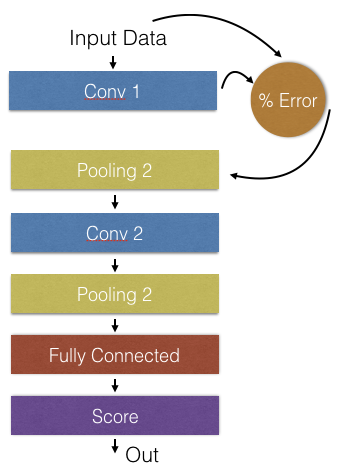
\includegraphics[width=0.3\textwidth]{Figure}
\end{figure}

\subsubsection{Mapping Floating point to Integer}
	\indent Caffe uses 32-bit floating point operations. ConvNets usually normalize their data values between 0 and 1 to keep the floating point numbers small. This can improve the performance of gradient descent during training. However, this means that the net has to perform operations in floating point. It does depend on the processor, but generally, floating point operations are slower and more power hungry than integer operations. We assume that for our application, there is no approximation during training, since it is very important that back-propagation in training be very accurate. Because approximation occurs only during testing and we have a good idea of the maximum values that the net will see, we can map from floating point to integer. Thus, we can take advantage of faster and lower power integer operations: a 32 x 32 bit integer approximate multiplier and a 32 bit approximate adder. We decided on a linear mapping of float to integer: $Integer=K*Float$ where $K$ is a power of 2 so that mapping can be implemented as shift. There are two sources of error from linearly mapping from floating point to integer. The first source of error is that floating point can represent extremely small values, but an integer mapping will have a quantization step size of $\frac{1}{K}$, but for a large K, quantization error will be small. The second error is that some valid input outside of our known data set could conceivably overflow our integer mapping and cause a very large error. The potential error is extremely large, so the mapping function is given some buffer room. The largest number that the float to integer mapping will represent is set at 16. We are doing signed 32-bit integer operations, so the largest positive number that we can represent is $2^{31}-1$. Therefore, to map $16.0\cdot K = 2^{31}-1$ results in $K = 2^{27}$. We used this K value for our power calculations and for our error approximation. 
	
\subsubsection{Mapping error from the adder}
\indent Error in the adder comes from the loss of carries propagating through the lower bits and the OR rather than an XOR operation which results in an underestimation. However, due to the carry in from the MSBs of the approximated bits, it is possible to overestimate, even without the carry propagating through the lower bits. The mean of the LOR approximate adder is -.25, but as is apparent in Figure 2, it has a very non-Gaussian spread, with a slight bias towards large positive errors and small but frequent negative errors. Thus, it is unlikely to get a mean as low as -.25 without adding every possible $2^{32}$ bit number, but the error still reduces the more numbers that are approximately summed together, which makes this added well suited to convNets. 

\indent Because we are using particular data as opposed to randomly distributed numbers, the error introduced to the convNet from the adder is strongly dependent on the value of $K=2^{27}$ and the spread of the input data. If the number of approximated bits becomes larger than $27$, then the addition becomes simply OR-ing together many bits, which results in an accumulation of ones in the lower bits rather than an accumulation in the typical summing sense. Thus the approximation gets drastically worse at and above 27 bits of approximation. 

\subsubsection{Mapping error from the multiplier}
\indent The multiplier approximates by zeroing out lower bits rather than calculating them. This results in mean and probability of error worse than our addition approximation. The error from approximation can be thought of as a floor rounding error. Because of this the multiplier error relies on the $K$ value significantly as well, since for large numbers of approximated bits the entire value can be rounded to zero. This occurs around 27 bits of approximation as well. 
 
\indent After a multiplication we get a 64-bit answer, which uses a $K^2$ term for mapping to floating point. Consider: $(A\times K) \times (B\times K) = (A\times B)K^2$. The right half of the equation can still be thought of as a floating point approximation, but with a quantization step of $\frac{1}{K^2}$. In the convolutional algorithm, after a multiplication an addition is performed. In this application, the addition is a 32-bit integer, which represents a floating point times K. Thus the $K^2$ term must become a $K$ term before the addition is performed by performing a 27-bit right shift. This conversion back to a 32-bit number could conceivably be a problem in a different application, since upper bits might be lost if the division by K is only a shift by 27 instead of a full 32. However, in our application this is not a problem, because all weight values $w$ are $|w|<1$. This means that our multiplier is very well suited to our application because we are already disregarding the lower 32 bits and we would like to waste as few resources on them as possible. 
	
\subsubsection{Introducing error into the convNet}
The convNet has three layers that are addition and multiplication intensive: convolution layer 1 ($conv_1$), convolution layer 2 ($conv_2$), and the fully connected layer ($fc_1$). Due to the labyrinthine nature of Caffe, it was outside of the scope of our project to implement an actual approximate adder and multiplier inside of the convNet code to judge the effect of approximation exactly. However, the python wrapper for Caffe is set up specifically to allow developers to examine and edit data in between layers. Thus, we introduce an estimated percent error at each of these layers as shown in Figure 1.

We obtain percent error individually for each layer, because each layer does a different number of operations on a different range of numbers. For example, to obtain error for the output of the $conv_2$ layer we ran 10000 training images through the un-approximated convNet and collected all of the $conv_2$ weights and 500000 non-zero sample numbers from the output of the $conv_1$ layer to serve as our expected input to the $conv_2$ layer. We ignored the output of the $pool_1$ pooling layer, because pooling throws away one fourth of the data. Layer $conv_2$ does a dot product between a weight matrix and a section of the output of $conv_1$. Therefore, to obtain an estimate of  error, we approximately multiply a weight with a data point and measure percent error. To introduce error into the convNet, a percent error is randomly selected from the sample error that was just generated for that layer and introduced to the output of $conv_2$ before it is passed on to the next layer.

The addition approximation error is obtained similarly, but it takes into account that there are multiple additions. Due to the nature of the LOR approximate adder, the mean error is very low, so it is an advantage that there are multiple approximated additions. For example, the $conv_2$ layer does a dot product between 25 numbers, so those 24 additions are likely to result in a lower error overall since the approximation is likely to over and underestimate and reduce some of the error. To account for this, addition percent error is calculated by approximately adding 25 numbers for both $conv_1$ and $conv_2$ and adding 80 numbers for $fc_1$. The sample numbers to be added are sampled inputs to a layer multiplied by random weights of that layer. This is to make sure that the sample addition is performed on the correct range. The percent error is obtained from these iterated additions and is introduced in between layers in the same way as the multiply. 

\section{Results}

\subsection{Hardware}
	\indent Figure 2 shows the power and area versus the number of bits approximated for the LPO adder. As the figure indicates, there is almost a linear relationship between the number of bits approximated versus power. Practically, this indicates that the optimal savings in power and area is linearly dependent on how much error the application can tolerate. Figure 3 shows how performance increases with number of bits approximated. It is important to note however, that this frequency is an estimate obtained from how much positive slack was obtained given a fixed period. Synopsys Design Compiler would need to be re-run at the optimal slack to obtain power and area specifications at that frequency. In this paper, we chose to use a fixed period in order to compare power and area metrics across different implementations of the adder. 	
\begin{figure}[t]
\caption{Num of Approximated Bits vs. Total Power and Area, Adder}
\centering
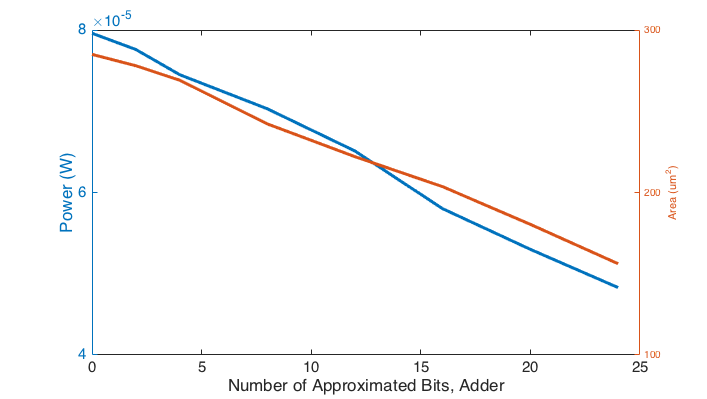
\includegraphics[width=0.50\textwidth]{Adder_PandA}
\caption{Num of Approximated Bits vs. Estimated Operating Freq, Adder}
\centering
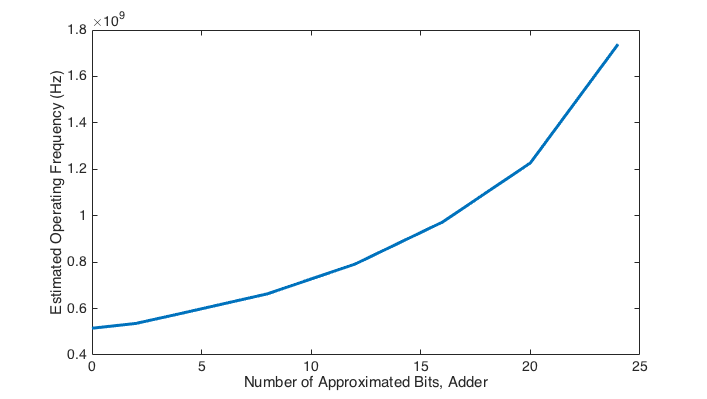
\includegraphics[width=0.50\textwidth]{Adder_OpFreq}
\end{figure}
\begin{figure}[t]
\caption{Num of Approximated Bits vs. Total Power and Area, Multiplier}
\centering
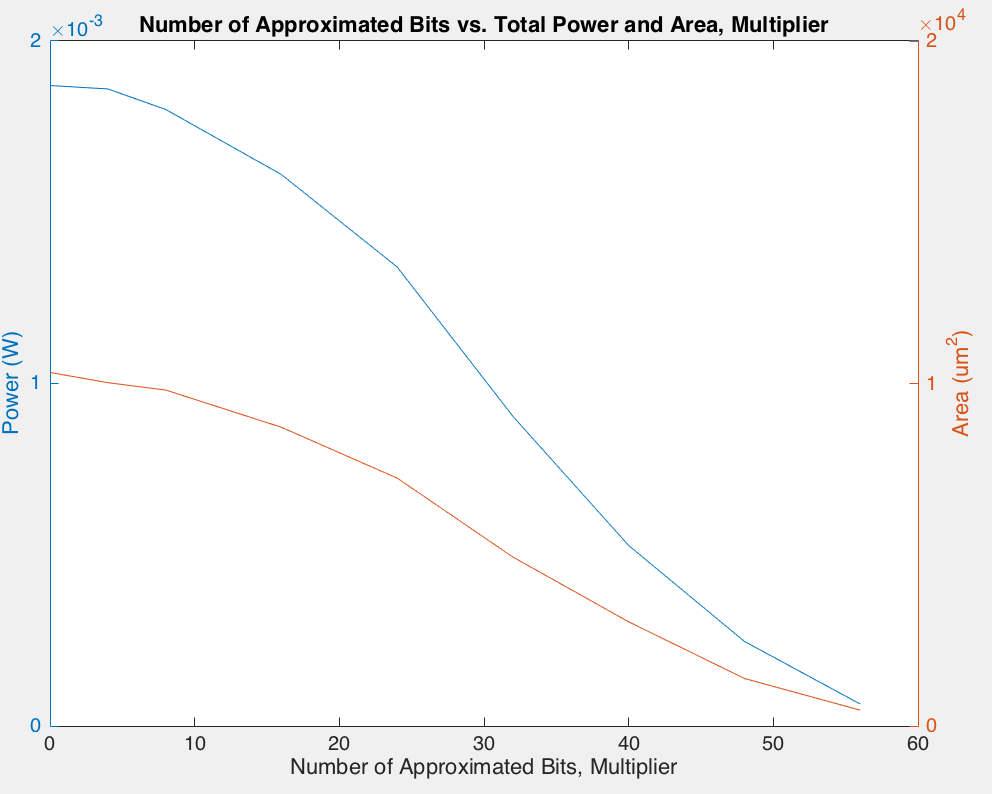
\includegraphics[width=0.50\textwidth]{Multiplier_PandA}
\caption{Num of Approximated Bits vs. Estimated Operating Freq, Multiplier}
\centering
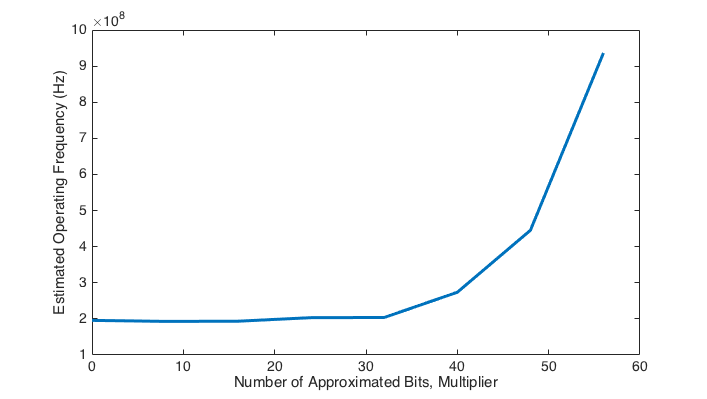
\includegraphics[width=0.50\textwidth]{Multiplier_OpFreq}
\end{figure}

	\indent Figure 4 shows the power and area versus vertical breaking line of the approximate multiplier. As expected, power and area are reduced as the vertical breaking line is increased. What is interesting to note, however, is the estimated operating frequency (Figure 5) barely changes when the vertical breaking line is under 30. Significant impact to the critical path only occurs at very high vertical breaking line values.

\subsection{ConvNet Accuracy}
	\indent We found that with proper selection of a $K$ value, convNet calculations can be significantly improve power, speed, and chip area without dramatically reducing neural net accuracy. The original accuracy of the net was $91.57\%$. The approximation was tested on exactly the same inputs to determine the change in accuracy resulting only from approximation as opposed to different inputs. For low numbers of bit approximation, the change in classification accuracy was less than a percent. In a few cases, the accuracy even increased by $.01\%$ due simply to a bit of fortunately placed error. This reinforces that error of less than $.01\%$ due to approximation is barely distinguishable from a functioning net.
	
	\indent The multiplier accuracy degraded convNet accuracy by less than a percent for up to 46 bits of approximation. Accuracy degraded by about $5\%$ at 50 bits of approximation, before accuracy plummeted, due to too many results being rounded down to zero. 
	
%		Mult
\begin{center}
 \begin{tabular}{||c|c||} 
 \hline
 Num Bits Approx & convNet Accuracy\\ [0.5ex] 
 \hline
	36& 0.9155 \\
 \hline
	38& 0.9158 \\
 \hline
	40& 0.9156 \\
 \hline
	42& 0.9167 \\
 \hline
	44& 0.9138 \\
 \hline
	46& 0.9120 \\
 \hline
	48& 0.8999 \\ 
 \hline
	50& 0.8655 \\ 
 \hline
	52& 0.7524 \\ 
 \hline
	54& 0.3742 \\ 
 \hline
\end{tabular} \\
\hfill \\
\bf{Multiply Approximated convNet Accuracy}
\end{center}

\indent For up to 4 bits of adder approximation, there was no measured change in the accuracy of the convNet. Like the multiplier, the accuracy of the convNet starts to decrease due to approximated addition error as the number of approximated bits becomes larger. However, the additions resulted in larger final answers, where as the multiplications with small layer weights resulted in smaller numbers which were more sensitive to error. Thus, the number of approximated bits for addition went up to 24 before convNet accuracy was reduced by more than a percent. However, there was also a drastic drop in error when the number of approximated bits surpassed the number of bits in a typically sized input. Indeed, with $K = 2^{27}$ and the average expected number around 1, the drastic drop in accuracy occurred exactly at 27 bits of approximation.
%		Adder
\begin{center}
 \begin{tabular}{||c|c||} 
 \hline
 Num Bits Approx & convNet Accuracy\\ [0.5ex] 
 \hline
	4& 0.9157 \\
 \hline
	8& 0.9155 \\
 \hline
	16& 0.915 \\
 \hline
	20& 0.9145 \\
 \hline
	24& 0.8917 \\
 \hline
	25& 0.8835 \\
 \hline
	26& 0.8657 \\ 
 \hline
	27& 0.3519 \\ 
 \hline
	28& 0.3519 \\ 
 \hline
\end{tabular} \\
\hfill \\
\bf{Add Approximated convNet Accuracy}
\end{center}

\indent Based on the adder and multiplier results individually, we ran various combinations to see the effect of both addition and multiplication error simultaneously. We found that we could achieve less than $1\%$ error with 46 out of 64 bits approximated in the multiplier and 20 out of 32 bits approximated in the adder.

%		both
\begin{center}
 \begin{tabular}{|l|c|c|c|c|c|c|c||} 
  \hline
 \theadfont\diagbox[width=4em, height=4em]{Add}{Mult}&
	\thead{36}&\thead{40}&\thead{44}&\thead{46}&\thead{48}&\thead{52}\\
 \hline
	\thead{4}& .9155 & X & .9138 & X & .8999 & X \\
 \hline
	\thead{8}& X & .9158 & X & .9120 & X & .7521 \\
 \hline
	\thead{16}& .9150 & X & .9140 & X & .9003 & X \\
 \hline
	\thead{20}& X & .9149 & X & .9106 & .8991 & .7516 \\
 \hline
	\thead{24}& .8912 & X & .8864 & .8821 & .8620 & X \\
 \hline
	\thead{26}& X & .8646 & X & .8449 & X & .1472 \\ 
 \hline
\end{tabular} \\
\hfill \\
\bf{Add and Multiply Approximated convNet Accuracy}
\end{center}

For each evaluation of one 28x28 image by the LeNet convNet, there are 408000 multiplications and 392780 additions. Using 46 bits approximated for the multiplier, and 20 bits for the adder, the average power savings obtained by extrapolating the above plots is almost 6.57X. Similarly, the area reduction is almost 6.77X that of a non-approximated adder and multiplier. 

\section{Conclusion}
	\indent ConvNets are a prevalent, power intensive applications, and based on our results they are also an excellent application for approximate computation. Approximate computing has shown improvements of almost 6.57X in power and 6.77X reduction in area using a vertical breaking line of 46 for multiplication and 20 bits of approximation in addition. This resulted in less than $1\%$ loss of accuracy in the LeNet classification. While it may not be worthwhile to implement specialized hardware in generalized consumer products, this work shows that for specialized cases where a convNet is well classified and power and area requirements are very important, approximation is a very powerful tool.

\begin{thebibliography}{1}

\bibitem{} A. Krizhevsky, I. Sutskever, G. E. Hinton, "ImageNet Classification with Deep Convolutional Neural Networks," Neural Information Processing Systems, pp. 1097–1105, 2012.	
\bibitem{} Y. Chen, T. Krishna , J. Emer, “Eyeriss: An Energy-Efficient Reconfigurable Accelerator for Deep Convolutional Neural Networks,” ISSCC 2016.
\bibitem{}H.R. Mahdiani, A. Ahmadi, S.M. Fakhraie, C. Lucas, “Bio-inspired imprecise computational blocks for efficient vlsi implementation of soft-computing applications,” IEEE Trans. Circuits and Systems I: Regular
Papers, vol. 57, no. 4, pp. 850-862, April 2010.
\bibitem{} K. Simonyan, A. Zisserman, “Very Deep Convolutional Networks for Large- Scale Image Recognition,” CoRR, 2014. 
\bibitem{} Otavio Good, “How Google Translate squeezes deep learning onto a phone,” Google Translate, July 29, 2015. http://googleresearch.blogspot.com/2015/07/how-google-translate-squeezes-deep.html
\bibitem{} Karpathy. A, "CS231n Convolutional Neural Networks for Visual Recognition," January, 2016. http://cs231n.github.io
\bibitem{} S. Venkataramani, “AxNN: Energy Efficient Neuromorphic System using Approximate Computing,” ISLPED 2014.
\bibitem{} K. Roy, A. Raghunathan, “Approximate Computing: An Energy-Efficient Computing Technique for Error Resilient Applications,” Computer Society Annual Symp. on VLSI, 2015.
\bibitem{}Farshchi, F, "New Approximate Multplier for Low Power Digital Signal Processing, " IEEE, 2013. 
\bibitem{} Sugawara, Y, "System for Automatic Generation of Parallel Multipliers over Galois Fields," IEEE, 2015.
'
%\bibitem{} LeCun, Y, "Gradient-Based Learning Applied to Document Recognition," IEEE, 1998.
%\bibitem{} J. Han, M. Orshansky, “Approximate Computing: An Emerging Paradigm For Energy-Efficient Design,” ETS, 2013.
%\bibitem{} S.-L. Lu, “Speeding up processing with approximation circuits,”Computer, vol. 37, no. 3, pp. 67-73, 2004.
%\bibitem{}N. Zhu, W.L. Goh and K.S. Yeo, “An enhanced low-power high-speed adder for error-tolerant application,” in Proc. ISIC’09, pp. 69–72, 2009.
%\bibitem{}N. Zhu, W.L. Goh and K.S. Yeo, “Ultra low-power high-speed flexible probabilistic adder for error-tolerant applications,” in Proc. Intl. SoC Design Conf., pp. 393–396, 2011.
%\bibitem{}J. Miao, K. He, A. Gerstlauer and M. Orshansky “Modeling and synthesis of quality-energy optimal approximate adders,” in Proc.ICCAD, pp. 728, 2012.
%\bibitem{}C. Lui, A Low-Power, "High-Performance Approximate Multiplier with Configurable Partial Error Recovery," EDAA, 2014.
%\bibitem{}Kyaw, K, "Low-Power High-Speed Multiplier For Error� Tolerant Application," EDSSC, 2010.


\end{thebibliography}
\begin{IEEEbiography}[{
\includegraphics[width=1in,height=1.25in,clip,keepaspectratio]{Emily_Pic}}]{Emily Naviasky}
Emily Naviasky earned a Bachelors in Electrical Engineering and in Computer Science at the University of Maryland. Presently, she is a Graduate Student at UC Berkeley interested in analog integrated circuits. She is upside-down, and has an innate resilience to imperfections in precision.
\end{IEEEbiography}

\begin{IEEEbiography}[{
\includegraphics[width=1in,height=1.25in,clip,keepaspectratio]{Keertana_Pic}}]{Keertana Settaluri}
is currently a first year doctoral student at UC Berkeley. She has gained immense popularity in the recent decade, and is small, practical, and well established. 
\end{IEEEbiography}

% You can push biographies down or up by placing
% a \vfill before or after them. The appropriate
% use of \vfill depends on what kind of text is
% on the last page and whether or not the columns
% are being equalized.

%\vfill

% Can be used to pull up biographies so that the bottom of the last one
% is flush with the other column.
%\enlargethispage{-5in}



% that's all folks
\end{document}


